\chapter{CPUの仮想化}
オペレーティングシステムは,
ハードウェアを抽象化した使いやすい拡張マシン(仮想マシン)を
必要な数だけ提供する.
数に限りがある資源が必要な数あるように見せるために仮想化が行われる.
CPU資源も仮想化し,
各プロセスが自分専用のCPUを持っているように見せかける.

\section{時分割多重}
CPUを仮想化するためには時分割多重が用いられる.
ハードウェアである実CPUの数は限られているので,
時間を区切って実CPUを使用するプロセスを次々に切換えていく.
\figref{virtualCPU}にCPU仮想化の原理を示す.

実CPUは\figref{cpuBlock}のような構造をもつハードウェアである.
プロセスの構造は\figref{procOrganization}に示した通りであり,
仮想CPUを含んでいる.
実CPUが短時間(例えば10ms)に次々と実行するプロセスを切換えていくことで,
複数のプロセスが夫々に専用のCPUを持ち並行して実行されているように見せかける.

まず,現在のプロセス実行中の実CPUのコンテキストを,プロセスの仮想CPU領域に保存する.
次に,新しく実行するプロセスの仮想CPU領域から実CPUにコンテキストを読込み,
新しいプロセスの実行を再開する.
一つのプロセスから別のプロセスに切換える処理を{\bf コンテキストスイッチ}と呼ぶ.
また,実CPUにコンテキストを読込んで実行を再開することを{\bf ディスパッチ},
ディスパッチを行うプログラムを{\bf ディスパッチャ}と呼ぶ.
\figref{osOrganization}にもディスパッチャは描かれていた.

\myfigure{btp}{scale=0.7}{virtualCPU-crop.pdf}
{時分割多重によるCPUの仮想化}{virtualCPU}

\section{プロセスの状態}
\label{procState}
プロセスは,
キーボード等の入出力装置からの入力を待つ状態になったり,
時間が経過するのを待つ状態になったりする.
{\bf 待ち(Waiting)状態}のプロセスにはCPUを割当てる必要がない.
このようにプロセスは幾つかの状態を持っている.
プロセスの状態はUNIXではpsコマンドで確認できる.
プロセスを模式的に示した\figref{procOrganization}では,
「プロセス情報」の「プロセスの状態」のことである.

\subsection{基本的な三つの状態}
\figref{procState}にプロセスの状態遷移図を示す.
この図は最も簡単なものであり,
実際のオペレーティングシステムでは,
もっと状態数が多くなる\footnote{
macOSのpsコマンドのオンラインマニュアルで確認すると,
macOSではプロセスの状態が,
I(Idle),
R(Runnable),
S(Sleep),
T(sTopped),
U(Uninterruptible wait),
Z(Zombi)の六つであることが分かる.}.
図に示された三つの状態を説明する.

\begin{itemize}
\item {\bf Ready(実行可能)} \\
CPUを割当てれば実行を開始できる状態のことである.
プロセスはCPUが割当てられるのを待っている.
\item {\bf Running(実行中)} \\
CPUが割当てられ実行している状態のことである.
CPUの数より多くのプロセスが同時にRunningになることはできない.
\item {\bf Waiting(待ち)} \\
シグナルの到着や入出力の完了等の事象を待っている状態である.
プロセスは実行することができない.
\end{itemize}

\myfigure{btp}{scale=0.66}{procState-crop.pdf}{プロセスの状態遷移}{procState}

\subsection{状態遷移}
\figref{procState}に示された六つの状態遷移の意味は以下の通りである.

\begin{enumerate}
\item {\bf Create(生成)} \\
新しいプロセスが生成されるとReady状態になる.
親プロセスが\|fork()|システムコール(UNIXの場合)や
\|CreateProcess()|システムコール(Windowsの場合)を実行すると,
新しい子プロセスが生成される.

\item {\bf Dispatch(派遣)} \\
Ready状態のプロセスは,
自分の順番が来たらCPUが割当てられRunning状態に遷移し実行を開始する.

\item {\bf Preemption(横取り)} \\
Running状態のプロセスは,
決められた時間(クオンタムタイム)を使い切ったとき,
より優先度の高いプロセスがReady状態になったとき等に,
CPUを取り上げられてReady状態に遷移する.

\item {\bf Block(事象待ち)} \\
Running状態のプロセスが,
システムコールを発行して自らWaiting状態に遷移することがある.
例えば入出力システムコール
(\|open()|,\|read()|,\|write()|,\|close()|等)や,
シグナル待ちシステムコール(\|pause()|,\|wait()|,\|sleep()|等)
を発行した場合である.
また,他のプロセスからシグナルを受信した場合も,
Waiting状態に遷移することがある.
更に,仮想記憶の機能を持つオペレーティングシステムでは,
プロセスが読み書きしようとした領域がメモリ上に存在しない時もこの遷移が起こり,
メモリ領域を確保するための処理がカーネル内部で始まる.

\item {\bf Complete(事象完了)} \\
Waiting状態のプロセスは,
入出力の完了やシグナルの発生等の事象(イベント)が発生すると
Ready状態に遷移する.
Waiting状態のプロセスは停止しているのでプロセスが事象を発生することはない.
事象はプロセスの外部からもたらされる.

\item {\bf Exit(終了)} \\
プロセスが自ら\|exit()|システムコール(UNIXの場合)や
\|ExitProcess()|システムコール(Windowsの場合)を用いて終了する場合,
プロセスがシグナルを受ける等して終了させられる場合に,
この遷移が起こる.
シグナルはプロセス(他プロセス,自プロセス)から明示的に送信される場合と,
自プロセスが保護違反などのエラーを起こして発信される場合がある.
\end{enumerate}

\section{プロセスの切換え}
Running状態のプロセスがBlock遷移またはPreemption遷移しCPUを取り上げられると,
他のReady状態のプロセスがCPUを割付けられDispatch遷移し実行される.

\subsection{切換えの原因}
Running状態のプロセスが状態遷移を起こす原因を以下にまとめ直す.

\begin{enumerate}
\item イベント \\
Running状態のプロセスは,
自ら「システムコールを発行」することでBlock遷移をすることがある.
また,他のプロセスからの「{\bf 干渉}\footnote{
干渉には,より優先順位の高いプロセスが実行可能になった,
別のプロセスからシグナル等を受取った等がある.}
を受け」Block遷移することがある.

\item タイムスライシング \\
Running状態のプロセスが長時間の実行を続けるとPreemption遷移をする.
一度に実行しても良い時間(クオンタムタイム)を使い切ったためである.
Ready状態のプロセスが他にあれば,そのプロセスに実行が切換わる.
他に実行すべきプロセスが無い場合は,再度,同じプロセスが実行される.
\end{enumerate}

\subsection{切換え手順}
\figref{procSwitch}に二つのプロセス間で実行が切り換わる様子を示す.
図では時間に従って上から下へ処理が進んでいく.
左側はプロセスAの実行を,
右側はプロセスBに実行を,
図の中央はカーネルの実行を表している.
プロセスの実行が切り替わっていく手順を以下で説明する.

\begin{enumerate}
\item 実行 \\
日頃はCPUがユーザ・プロセスを実行している.

\item 割込み \\
割込みが発生し処理がプロセスAからカーネル内の割込みハンドラに移る.
割込みの原因は\ref{interruptSource}で述べた様々な原因が考えられる.
割込みが発生すると以下の処理が{\bf CPUのハードウェアにより自動的に}される.
\begin{enumerate}
\item CPUの(PCを含む)PSWがスタックに保存される.
\item CPUの実行モードがカーネルモードに切り換わる.
\item 割込みハンドラにジャンプする.
\end{enumerate}

\item 割込みハンドラ \\
PSW(スタック上にある)とCPUレジスタ(\figref{cpuBlock}参照)からなる
プロセスのコンテキストを
プロセスの仮想CPU領域(\figref{procOrganization}参照)に保存する.
次に割込み原因を調べ,
割込み原因に応じた処理(サービスモジュール等)にジャンプする.
例えば,
割込み原因が\|open()|システムコールなら,
openシステムコールの処理を行うファイルシステムの
サービスモジュールにジャンプする.
割込み原因がI/O完了なら,完了したI/Oに対応するデバイスドライバにジャンプする.

\item サービスモジュール等 \\
割込み原因に応じた処理を行う.
この過程でプロセスの状態が変化させることがある.
例えば,プロセスが発行したシステムコールが原因でBlock遷移する場合や,
タイマーやI/Oの完了割込によりWaiting状態だった別のプロセスが
Complete遷移する場合,
タイマーの完了割込により現在のプロセスがPreemption遷移する場合等が考えられる.
サービスモジュールの処理が完了するとディスパッチャにジャンプする.

\item ディスパッチャ \\
実行可能なプロセスの中から適切な一つを選び,
選んだプロセスの仮想CPU領域の内容をCPUレジスタにロードする.
最後にPSWを復旧する機械語命令を実行しコンテキストを完全にCPUにロードし,
プロセスの実行に戻る.
CPUの実行モードを表すフラブはPSWに含まれているので,
PSWが復旧されることで実行モードがカーネルモードからユーザモードに切り換わる.
PSWを復旧する機械語命令として割込復帰用の{\bf RETI
(RETurn from Interrupt)命令}を用いる.
RETI命令は単一の命令でPSW(PCとフラグ)を一度にスタックから復旧する.

\item 実行 \\
新しく選択されたユーザ・プロセスが実行される.
\end{enumerate}

\figref{procSwitch}の下半分,
プロセスBからプロセスAへ実行が移る手順も上と同様である.

\myfigure{btp}{scale=0.6}{procSwitch-crop.pdf}{プロセスの切換え}{procSwitch}

\subsection{切換えの例}
計算に長い時間を要する二つのプロセスだけがある時,
クオンタムタイムを使い切ってもう一方のプロセスに切り換わり,
交互に実行される様子を\figref{procSwitchInst}に示す.
以下に手順を説明する.

\myfigure{btp}{scale=0.6}{procSwitchInst-crop.pdf}
{プロセスの切換えの例}{procSwitchInst}

\begin{enumerate}
\item 実行 \\
プロセスAは計算処理を続けている.
長い時間に渡ってシステムコールを発行することは無い.

\item タイマー割込み \\
タイマーは一定間隔で割込みを発生する.
割込が発生するとCPUのハードウェアが自動的にPSWを保存し,
割り込みハンドラにジャンプする.
オペレーティングシステムは,
主に,この割込みを基準に時間の経過を認識する.

\item 割込みハンドラ \\
プロセスのコンテキストをプロセスの仮想CPUに保存する.
その後,割込原因を調べタイマーからの割込みなので,
「タイマーに関する処理」を行うカーネル内のモジュールへジャンプする.

\item タイマーに関する処理 \\
一定間隔で発生するタイマーからの割込みを利用して,
システムの時計を進めたり,
リソース(CPUやメモリ等)の利用統計データを更新したりする.
その間にプロセスAがクオンタムタイムを使い切ったことが判明すると,
プロセスAをPreemption遷移させる.
この時点でプロセスAの状態がReadyに変化する.

\item ディスパッチャ \\
Ready状態のプロセスの中から適切な一つを選びDispatch遷移させる.
\figref{procSwitchInst}はプロセスBが選択された場合である.
ディスパッチャはプロセスBのCPUレジスタを復旧する.

\item RETI \\
プロセスBのPSWを復旧し,プロセスBの実行を再開する.

\item 実行 \\
プロセスBは計算処理を再開する.
プロセスBも長い時間計算を続けるプロセスとする.

\item タイマー割込み \\
計算を続けるうちにタイマーからの割込みが発生する.

\item 割込みハンドラ \\
プロセスBのコンテキストを保存する.

\item タイマーに関する処理 \\
プロセスBは,まだ,クオンタムタイムを使い切っていないので,
Preemptionは発生しない.

\item ディスパッチャ \\
Preemptionは発生しないので,
プロセスBのコンテキストを復旧する.

\item RETI \\
プロセスBに戻る.

\item 実行 \\
プロセスBは計算処理を再開する.

\item タイマー割込み \\
8.〜13. を何度か繰り返し,
クオンタムタイムを使い切った時のタイマー割込みである.

\item 割込みハンドラ \\
プロセスBのコンテキストを保存する.

\item タイマーに関する処理 \\
クオンタムタイムを使い切ったのでPreemptionが発生する.

\item ディスパッチャ \\
Ready状態のプロセスAを選択しDispatch遷移させる.
プロセスAのコンテキストを復旧する.

\item RETI \\
プロセスAに戻る.

\item 実行 \\
プロセスAは計算処理を再開する.
\end{enumerate}

\section{PCB(Process Control Block)}
PCBはプロセス毎に用意される最も重要なカーネルのデータ構造である.
PCBはカーネル内のプロセステーブルに格納される.

\subsection{PCBの内容}
PCBは,\figref{procOrganization}に示した模式的なプロセスの構造図の
「仮想CPU」と「プロセス情報」を合わせたものに相当する.
PCBには以下のような情報が格納される.

\begin{itemize}
\item 仮想CPU
\item プロセス番号
\item 状態(Running,Waiting,Ready等)
\item 優先度
\item 統計情報(CPU利用時間等)
\item 次回のアラーム時刻
\item 親プロセス
\item 子プロセス一覧
\item シグナルハンドリング
\item 使用中のメモリ
\item オープン中のファイル
\item カレントディレクトリ
\item プロセス所有者のユーザ番号
\item PCBのリストを作るためのポインタ
\end{itemize}

\subsection{PCBリスト}
PCBはプロセスを表現するデータ構造である.
例えば,Ready状態のプロセスは優先度順にソートされ,
優先順位が最も高いものから順にCPUが割当てられる.
ソートされたReady状態のプロセスのリストは,
優先度をキーにソートされたPCBの線形リスト(待ち行列)として表現される.
その様子を\figref{procQueue}に示す.
図は,数値が小さいほど優先度が高い意味になっている.

\myfigure{btp}{scale=0.55}{procQueue-crop.pdf}{PCBのリスト}{procQueue}

Ready状態のプロセスだけでなく,
Running状態のプロセスや,
Waiting状態のプロセスも待ち行列として表現される.
Waiting状態のプロセスは,
待ち合わせているイベント毎に待ち行列を作っている.
イベント待ちの待ち行列のソート順はイベント毎にルールが決められる.

プロセスの状態遷移に合わせてPCBが待ち行列の間を移動する.
\figref{procQueue}の左側の「状態遷移と待ち行列の移動」が
「どの待ち行列から,どの待ち行列に移動可能か」を表している.
例えば,Running状態(実行中)のプロセスがPreemption遷移をすると,
状態がReadyに変わるだけでなく,
PCBが「実行可能なプロセスの待ち行列」に移動する.
この移動ルールは\figref{procState}の状態遷移と一致している.

\section{TacOSのCPU仮想化}
実例としてTacOS\footnote{TacOSの詳細は
\url{https://github.com/tctsigemura/TacOS}
を参照のこと.}の例を紹介する.
TacOSはマルチプロセスのオペレーティングシステムである.
以下ではCPUの時分割多重に必要なプロセス切換え機構を紹介する.

\subsection{PCB}
PCBはプロセス切換え機構にとっても最も重要なデータ構造である.
TacOSのPCBは\figref{tacosPCB}に示す\|PCB|構造体として定義されている\footnote{
\figref{tacosPCB}はTacOSのソースコード
\url{https://github.com/tctsigemura/TacOS/blob/master/os/kernel/process.h}
の一部である.}.
\|PCB|構造体の内容を順に説明する.

\begin{figure}[btp]
\lstinputlisting{Lst/pcb.hmm}
\caption{TacOSのPCB宣言ソースプログラム}
\label{fig:tacosPCB}
\end{figure}

\begin{itemize}
\item 仮想CPU(\|sp|) \\
TacOSはプロセスのコンテキストのほとんどをカーネルスタック上に保存する.
そして,保存位置を表すスタックポインタ(SP)だけをPCBに保存する.
PCBに保存されるのは仮想CPUの一部だけである.

\item プロセス番号(\|pid|)

\item 状態(\|stat|) \\
TacOSのプロセスの状態は以下の三つである.
\begin{enumerate}
\item \|P_RUN| \\
RunningとReadyの二つを兼用している.
プロセスは実行可能プロセスの待ち行列(実行可能列)に挿入される際に
\|P_RUN|状態になる.
実行中も\|P_RUN|状態のまま変更しない.

\item \|P_WAIT| \\
Waiting状態のことである.

\item \|P_ZOMBIE| \\
プロセスが終了したが,終了ステータスを親プロセスに渡していない状態である.
終了処理の途中状態と考えるとよい.
\end{enumerate}

\item 優先度(\|nice|,\|enice|) \\
ゼロが最も高い優先度を表す.
優先度には,
本来の優先度(\|nice|)と,
実質の優先度(\|enice|)の二つがある.
現在の実装ではこの二つは同じ値を持つ.
将来,動的に変化する優先度を採用する場合に,
\|enice|の値が変化するようにする.

\item プロセステーブルのインデクス(\|idx|) \\
このPCBが登録されているプロセステーブル内の位置である.
プロセスが消滅する際にプロセステーブルからPCBを削除するために使用する.

\item イベント用カウンタとセマフォ(\|evtCnt|,\|evtSem|) \\
セマフォはプロセス間の同期に使用する基本的な機構である\footnote{
詳しくは後の章で解説する.}.
タイマー待ち,子プロセスの終了待ち等で,
このセマフォを使用してプロセスを待ち状態にする.
カウンタはタイマーの待ち時間を計るため等に使用される.

\item プロセスのアドレス空間(\|memBase|,\|memLen|) \\
TacOSには仮想記憶のような高度な機構は無い.
各プロセスは,
物理メモリの領域をオペレーティングシステムによって割付けられる.
\|memBase|は
オペレーティングシステムがプロセスに割当てたメモリ領域の開始アドレス,
\|memLen|はメモリ領域のバイト数である.

\item プロセスの親子関係の情報(\|parent|,\|exitStat|) \\
TacOSのプロセスは親プロセスだけ記憶している.
\|parent|は親プロセスのPCBを指すポインタである.
\|exitStat|は\|P_ZOMBIE|状態になった時,
親に渡すべき終了ステータスを保存する領域である.

\item オープン中のファイル一覧(\|fds|) \\
プロセスがオープンしたファイルのファイルディスクリプタ(番号)の
一覧を記憶する配列である.
TacOSではシステム全体で一意なファイルディスクリプタ(番号)が
用いられる\footnote{
UNIXのファイルディスクリプタ(番号)はプロセス毎に0番から割振られる.}.
\|close()|システムコールは,
クローズするファイルディスクリプタが正当なものか調べるために,
この配列を使用する.
\|exit()|システムコールは,
プロセスを終了する前にプロセスの全オープンファイルをクローズするために,
この配列を使用する.

\item PCBリストの管理(\|prev|,\|next|) \\
TacOSはプロセスのリストをPCBのリストとして表現する.
TacOSのPCBリストは番兵付きの重連結環状リストである
(\figref{tacosReadyQueue}参照).
\|prev|,\|next|はリスト上で前後のプロセスのPCBを指すポインタである.

\item スタックオーバーフローの検知(\|magic|) \\
TacOSはPCBの直後にプロセスのカーネルスタックを配置する.
万一,カーネルスタックがオーバーフローするとPCBが後ろから破壊される.
\|magic|はそれを検知するために使用される.
TacOSはPCBを初期化する際に\|magic|に\|0xabcd|を格納する.
カーネルスタックがオーバーフローすると,まず,\|magic|領域が破壊される.
\|magic|の値が変化していないかチェックすることで,
カーネルスタックのオーバーフローを検知することができる.
\end{itemize}

\subsection{メモリ配置}
\figref{tacosMemMap}にTacOS実行時のメモリマップを示す.
図は二つのプロセスが実行中の例である.
まず「物理メモリ空間」の配置について,
次に「PCBとカーネルスタック」について説明する.

\myfigure{btp}{scale=0.6}{tacosMemMap-crop.pdf}
{TacOSのメモリ配置}{tacosMemMap}

\begin{enumerate}
\item[(a)] 物理メモリ空間

\begin{itemize}
\item カーネル \\
カーネルのプログラムとデータ(変数)がこの領域に配置される.

\item プロセス#1のPCBとカーネルスタック \\
プロセス1のPCBとカーネルスタックが隣接して配置される.
詳細は\figref{tacosMemMap}(b)に示してある.

\item プロセス#2のPCBとカーネルスタック \\
プロセス毎にPCBとカーネルスタックが準備される.

\item プロセス#1のメモリ空間 \\
プロセス1のプログラム,データ,ヒープ,スタック領域が配置される.
ユーザモードのプロセスは,
この範囲以外のメモリをアクセスできないように保護すべきである.
しかし,TaCはメモリ保護機構を持っていない.

\item プロセス#2のメモリ空間 \\
プロセス毎にメモリ空間が準備される.
\end{itemize}

\item[(b)] PCBとカーネルスタック \\
PCBとカーネルスタックはプロセスの生成時に隣接して領域が確保される.
ユーザプログラム実行中はスタックの内容が空になる
(スタックポインタがスタック領域の最大アドレスを指す.).
割込みが発生すると自動的にPSWがカーネルスタックに保存され,
実行モードがカーネルモードに切換わる.
次に割込みハンドラに制御が移りCPUレジスタをスタックに保存した後,
カーネル内ルーチンの実行が始まる.
カーネル内ルーチンは,PCBに向かって伸びるカーネルスタックを使用する.
そこで,PCBの最もスタック寄りにマジックナンバー(\|0xabcd|)を配置し,
スタックが伸びすぎPCBを破壊したことを検知するために使用する.
\end{enumerate}

\subsection{プロセス切換えプログラム}
\figref{tacosDispatcher}にTacOSのプロセス切換えプログラムを示す
\footnote{\figref{tacosDispatcher}はTacOSのソースコード
\url{https://github.com/tctsigemura/TacOS/blob/master/os/kernel/dispatcher.s}
の一部である.プログラムはTaCのアセンブリ言語で記述してある.}.
切換えプログラムは,
コンテキストを保存する\|yield()|\footnote{
高級言語から{\tt yield()}関数を呼出すと,
アセンブリ言語の{\tt \_yield}ルーチンが実行される.}
と復旧する\|dispatch()|\footnote{
高級言語から{\tt dispatch()}関数を呼出すと,
アセンブリ言語の{\tt \_dispatch}ルーチンが実行される.}
からなる.
\|dispatch()|は
\figref{tacosReadyQueue}に示す実行可能列の先頭プロセスを実行する.
TacOSは,PCBを実行可能列に置いたままプロセスを実行する.
TacOSは,\figref{tacosMemMap}(b)に示すように,
プロセス毎にユーザモードとカーネルモードの二つのコンテキストを保存する.

割込が発生しカーネル内に実行が移ると,
まず,割込みハンドラがユーザモードのコンテキストをカーネルスタックに保存する.
次に,カーネルモードでカーネル内のプログラムが実行される.
この時点では,割込み前のプロセスの一部として実行されている.
プロセスを切換えるためには\|yield()|を呼出す.
\|yield()|はカーネルモードのコンテキストをカーネルスタックに追加保存し,
新しいプロセスの実行に切換える.
次回,プロセスの実行が再開されるのは,
カーネル内の\|yield()|を呼出した位置になる.
次に\figref{tacosDispatcher}の内容を解説する.

\myfigure{btp}{scale=0.6}{tacosReadyQueue-crop.pdf}
{TacOSの実行可能列}{tacosReadyQueue}

\begin{description}
\item[2行] プロセスを切換える時にカーネル内で呼出される\|yield()|関数の入口である.
\|yield()|関数は,現在プロセスのカーネルモード・コンテキストを保存しCPUを解放する.

\item[3〜16行] プロセスのカーネルモードのコンテキストを
スタックに保存する処理である.
\|yield()|が(CALL命令で)呼出された時点でPCはスタックに格納されている.
後でRETI命令でPCとFLAGを同時に復旧するのでPCの次にFLAGを格納している
(7行,\figref{tacosMemMap}(b)参照)).

\item[17〜19行] プロセスのカーネルモードのコンテキストを
保存したスタックの位置をPCBに保存する.
\|_curProc|変数には現在のプロセスのPCBを指すポインタが保存されている
(\figref{tacosReadyQueue}参照).
PCB先頭の\|sp|領域(\figref{tacosPCB}参照)にスタックポインタを保存する.
ここまでの処理でコンテキストの保存が完了した.

\item[20〜23行] カーネルスタックがオーバーフローしていないか調べる.
PCBの\|magic|フィールドの値をチェックし\|0xabcd|以外の値になっていたら,
カーネルスタックが隣接するPCBまで伸びた(オーバーフローした)と判断する.
この場合,\|.stkOverFlow|ルーチンにジャンプしシステムを停止する.
カーネルのエラーなので復旧は諦める.
オーバーフローが検知されない場合は26行に進み,
新しいプロセスにディスパッチする.

\item[26行] プロセスにCPUを割り付ける
ディスパッチャ(\|dispatch()|関数)の入口である.

\item[27〜31行] まず,
実行可能列(\|_readyQueue|)の先頭プロセスのPCBアドレスを
\|_curProc|変数にセットする.
実行可能列は番兵付きの重連結環状リストなので番兵の次が先頭のPCBである
(\figref{tacosReadyQueue}参照).
実行可能なプロセスが無い場合はidleプロセスが選択される.
\|_curProc|が更新されたので,新しいプロセスが現在のプロセスになった.
次に,現在のプロセスの保存してあったスタックポインタ(\|sp|)を復旧する.

\item[31〜42行] スタックポインタが復旧されたので,
スタックからCPUレジスタを復旧する.

\item[43〜44行] RETI命令を用いてPSW(FLAGとPC)を復旧し,
前回プロセスが\|yield()|を呼出した位置に戻る.
\|yield()|を呼出した位置に戻るためにRET命令ではなくRETI命令を使用するのは,
プロセス生成時は例外的に,
このRETIで実行モードを切換えてユーザプログラムの実行を開始するからである.
\end{description}

\begin{figure}[btp]
\lstinputlisting{Lst/dispatch.s}
\caption{TacOSのプロセス切換えプログラム}
\label{fig:tacosDispatcher}
\end{figure}

\section{スレッド(Thread)}
ここまで,一つのプロセスが一つの仮想CPUを持つモデルを考えてきた.
しかし,実際のコンピュータのハードウェアはCPUを複数持つ場合がある.
これでは
「ハードウェアの機能を抽象化した便利な{\bf 拡張マシン}」
(\ref{abstruction}参照)であるはずのプロセスが,
「CPUが一つしかない{\bf 縮小マシン}」なっている.
そこで,プロセスが複数の仮想CPUを持つモデルを導入する.
これにより,一つのプロセスに
並列実行する複数の処理の流れ(スレッド)を持つことが可能になる.

\subsection{スレッドの役割}
複数のプロセス(ジョブ)を主記憶にロードしておくことで
CPUの利用効率を高くできることは既に説明した
(\pageref{multiprogramming}ページ,マルチプログラミング参照).
マルチプログラミングの,もう一つのメリットは,
プログラミングが簡単になる場合があることである.
以下ではWebサーバを例に,
マルチプログラミングによる改善を紹介する.


\begin{itemize}
\item マルチプロラミングなし \\
\figref{singleProcSingleThread}(a)に最も簡単なモデルを示す.
Webサーバはリクエストを受信すると,それに対するレスポンスを返す.
処理は1番目のクライアントから順に行われ,
2番目のクライアントは1番目の処理が終了するまで待たされる.
このモデルの問題点は,
処理中にWebサーバプロセスがI/O待ち等でブロック(Block)する可能性があり,
その間,他のクライアントへのサービスがされないことである.

2番目以降のクライアントが長時間待たされないように,
複数のクライアントの処理を並行してできるように改良したモデルが
\figref{singleProcSingleThread}(b)である.
「I/O完了の監視」は通信を含む複数の入出力を同時に監視し,
どれかが読み書き可能になるのを待つ機能である.
UNIXでは\|select()|システムコールがこの機能を持つ.
読み書き可能になったことを確認後に読み書きを行うので
プロセスがブロックすることが無くなり,
複数のクライアントに対して同時にサービスを行うことができる.

しかし,Webサーバのプログラミングは難しくなる.
一方のクライアントの処理が終わらないうちに,
別のクライアントの処理を開始する必要があるからである.
クライアント毎に処理がどこまで進んでいるのかを表す{\bf 状態}を持つ必要がある.
また,CPUが複数存在する場合でも,
同時には一つのCPUしか働かないことも問題である.

\begin{myfig}{btp}{マルチプログラミングを用いないWebサーバ}
{singleProcSingleThread}
\begin{center}
\myincludegraphics{singleProcSingleClient-crop.pdf}{scale=0.6}

\vspace{0.8cm}

\myincludegraphics{singleProcMultiClient-crop.pdf}{scale=0.6}
\end{center}
\end{myfig}

\item マルチプロセス \\
マルチプログラミングを用いることで前記の問題を解決したモデルを
\figref{multiProc}(a)に示す.
Webサーバプロセスは,
まず,接続要求を待ちクライアント1からの接続を受け入れる.
次に,クライアント1専用のサーバプロセスを生成し処理を任せる.
Webサーバプロセスは,
生成したプロセスの終了を待たずに,
次の接続要求待ちになる.
クライアント2からの接続要求があったら
クライアント2専用のサーバプロセスを生成し,
接続要求待ちに戻る.

このモデルなら,
各クライアントの処理を別々のプロセスが行っているので,
プロセスがブロックしても構わない.
そのため,プログラミングは簡単になる.
また,CPUが複数あればプロセスが真に並列に実行される.
しかし,プロセスの生成はメモリ空間の確保や初期化を含み{\bf 重い処理}である.
また,プロセスはメモリを共有していないのでプロセス間の情報共有には効率が悪い.

\item マルチスレッド \\
複数のスレッドを使用したモデルを\figref{multiProc}(b)に示す.
マルチプロセスの場合と良く似たプログラムであるが,
クライアント毎に専用のプロセスを作る代わりに,
クライアント毎に専用のスレッドを作る.
スレッドの生成はプロセス生成より10〜100倍速いと言われている\cite{lightWeight}.
また,スレッドはメモリを共有しているので情報共有には都合が良い.
例えば,Webサーバが頻繁に参照されるページをメモリ上にキャッシュする場合,
キャッシュをスレッドで共有できる.
\end{itemize}

\begin{myfig}{btp}{マルチプログラミングを用いるWebサーバ}{multiProc}
\myincludegraphics{multiProc-crop.pdf}{scale=0.6}

\vspace{0.8cm}

\myincludegraphics{multiThread-crop.pdf}{scale=0.6}
\end{myfig}

\subsection{スレッドの形式}
読者は,「スレッドはカーネルが実現する」と暗黙のうちに考えていたかも知れない.
しかし,ユーザプログラム(ライブラリ)内でスレッドを実現することもある.
カーネルが実現するスレッドを{\bf カーネルスレッド},
ユーザプログラム内で実現するスレッドを{\bf ユーザスレッド}と呼ぶ.

\begin{myfig}{btp}{ユーザスレッドとカーネルスレッド}{threadOrganization}
\myincludegraphics{kernelThread-crop.pdf}{scale=0.6}

\vspace{0.8cm}

\myincludegraphics{userThread-crop.pdf}{scale=0.6}
\end{myfig}

\begin{itemize}
\item カーネルスレッド \\
カーネルスレッドの模式図を\figref{threadOrganization}(a)に示す.
カーネルスレッドはプロセスの仮想CPUを複数にし,
仮想CPUがプログラムを並行して実行する.
「プロセス情報」から「プロセスの状態」は無くなり,
代わりに仮想CPU毎に「仮想CPUの状態」を管理するようになる.
CPUが複数ある時,カーネルスレッドであれば,
プロセス内を真に並列実行することが可能である.

\item ユーザスレッド \\
ユーザスレッドの模式図を\figref{threadOrganization}(b)に示す.
プロセスには単一の仮想CPUしかない.
ユーザスレッドは仮想CPUを時分割多重して実現される.
カーネルを経由しないでスレッドの生成や切換えをすることができるので,
オーバーヘッドが非常に小さい.
\end{itemize}

以下に述べるように,両者を組合せた三つのスレッドモデルが使用される.

\begin{enumerate}
\item {\bf Many-to-One Model} \\
複数(Many)のユーザスレッドを
一つ(One)のカーネルスレッドで実行するモデルである.
\figref{threadOrganization}(b)に相当する.
プロセス内にカーネルスレッドは一つしか存在しない.
ユーザスレッドはユーザプログラム(ライブラリ)の工夫で
単一のカーネルスレッドを複数に見せかけているだけなので,
真の並列実行にはならない.
また,何れかのスレッドがシステムコールでブロックすると,
全てのスレッドが停止してしまう問題がある.

\item {\bf One-to-One Model} \\
全てのスレッドがカーネルスレッドのモデルである.
\figref{threadOrganization}(a)に相当する.
プロセス内にカーネルが管理する仮想CPUが複数あるので,
複数プロセスと同等な並列実行が可能である.
しかし,スレッドの生成や切換えにカーネルが介入するので,
処理は重くなる.
また,システムによっては生成できるスレッド数に制限がある.

\item {\bf Many-to-Many Model} \\
複数の(Many)のユーザスレッドを
複数の(Many)のカーネルスレッドで実行するモデルである.
カーネルスレッドの数をユーザスレッドの数より多くすることはない.
前記二つのモデルの折衷案である.
\end{enumerate}

\subsection{スレッドプログラミング}
配列データの合計を求める処理をスレッドを用いて高速化する例を考えよう.
\figref{threadedSum}に原理を示す.
配列aをM分割し個別スレッドで(CPUが複数あれば)同時に小計を計算する.
小計は配列totalに格納する.
最後にmainスレッドがtotalの合計を求めると全体の合計sumが計算できる.

\myfigure{btp}{scale=0.66}{threadedSum-crop.pdf}
{M個のスレッドで手分けして合計を計算する様子}{threadedSum}

\subsubsection{POSIXスレッドによる実装}
このアイデアをPOSIXスレッド\footnote{
POSIXスレッドはUNIX系のオペレーティングシステムで使用できる.
}を用いたC言語プログラムにしたものを\figref{threadTest}\footnote{
このプログラムは macOS High Sierra で動作確認をした.
}に示す.

\begin{figure}[btp]
\lstinputlisting{Lst/threadTest.c}
\caption{M個のスレッドで分担して配列データの合計を求めるプログラム}
\label{fig:threadTest}
\end{figure}

12行の\|thread()|関数はM個のスレッドで同時に並列実行される.
配列\|a|の担当範囲等は引数\|arg|により指示される.
関数の引数(\|arg|)やローカル変数(\|args|,\|sum|,\|i|)は,
スレッドのスタック(\figref{threadOrganization}参照)に割り付けられるので,
スレッド毎に別の実体を持つ.
グローバル変数\|a|や\|total|等は全てのスレッドで共有される.

33行の\|pthread_attr_init()|は引数の\|pthread_attr_t|型変数を
デフォルトのアトリビュート値で初期化する.
34行の\|pthread_create()|がスレッドを生成する関数である.
新しいスレッドの実行は引数で指定された\|thread()|関数から始まる.
\|pthread_create()|の引数\|p|は,
\|thread()|関数が実行を開始する時に\|arg|引数に渡される.

39行の\|pthread_join()|はスレッドの終了を待つ関数である.
スレッドの終了が確認できたら,40行で小計を\|sum|に足し込んでいる.

\subsubsection{実行時間の計測結果}
\figref{threadTest}のプログラムの実行時間の計測結果を\tabref{threadTimeTbl}に,
グラフにしたものを\figref{threadTimeGrph}に示す
\footnote{
実行時間の計測にはOS X の {\tt time} コマンドを用いた.
}
\footnote{
実行時間が短すぎて比較し難いので,
プログラムの14行から17行を10万回繰り返すように改造した上で計測した.}
\footnote{
計測に使用したコンピュータは
OS X Yosemite をインストールした
Mac Pro(Late 2013, 3.5GHz 6-Core Intel Xeon E5)である.
%macOS High Sierra をインストールした
%MacBook Pro(Retaina, 13-inch, Mid 2014, 2.8GHz Intel Core i5)である.
C言語コンパイラは
Apple LLVM version 7.0.0(clang-700.0.72)を使用した.
}.

\begin{mytable}{btp}{スレッド数による実行時間比較}{threadTimeTbl}
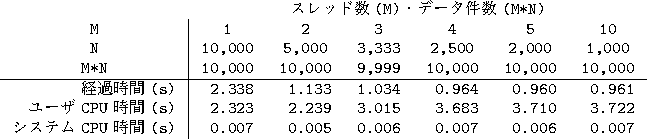
\includegraphics[scale=0.9]{Tbl/threadTimeTbl.pdf}
\end{mytable}

\begin{myfig}{btp}{スレッド数による実行時間の変化}{threadTimeGrph}
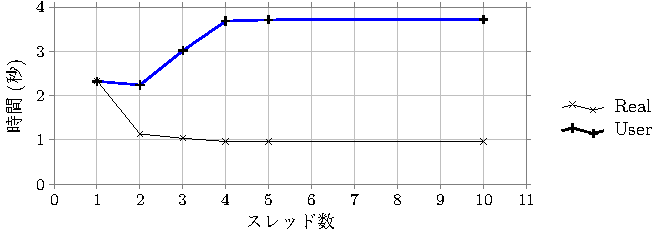
\includegraphics[scale=1.0]{Tbl/threadTimeGrph.pdf}
\end{myfig}

スレッド数が1の時は,経過時間(Real)とユーザCPU時間(User)が,
ほぼ,同じになる.
一つのコア\footnote{従来のCPUのこと.}が全力で合計を計算した結果である.

スレッド数が1〜6の間は,経過時間がスレッド数に反比例して短くなる.
合計の計算時間に対応するユーザCPU時間は,ほぼ一定である.
使用したコンピュータが持つ六つのコアが,
最大で六つのスレッドに割当てられ,
真に並列実行された結果である.

スレッドの数が6〜10に増加する間,経過時間は,ほぼ一定である.
しかしユーザCPU時間が増加している.
必要な計算量は一定のはずなのに長いCPU時間を必要とするので,
コアの性能が悪化したように見える.

コアの性能が悪くなったように見えるのは,
ハイパースレッディング・テクノロジー\cite{hyperThreading}により,
コアの数が倍(12個)あるように見せかけているためである.
ハイパースレッディング・テクノロジーは,
単一スレッドを実行する場合は遊んでしまうコア内のユニットを,
二つのスレッドを同時に実行することで効率よく使用する技術である.
見かけ上コアの数が二倍になるが,合計の性能は二倍には達しないので,
コアあたりの性能が下がったように見える\footnote{
この計測結果からは,
ハイパースレッディング・テクノロジーは,
性能の改善に余り寄与していないように見える.
}.

%スレッド数を12以上にすると,
%(見かけ上の)コア全てが常時使用されるので,
%経過時間,ユーザ時間の合計のどちらも一定になる.

